\documentclass[12pt,a4paper]{cibb}

\usepackage{subfigure,graphicx}
\usepackage{amsmath,amsfonts,latexsym,amssymb,euscript,xr}
\usepackage{multirow}
\usepackage{hyperref}
\usepackage{svg}

\title{\large $\ $\\ \bf ON SECONDARY STRUCTURE ANALYSIS BY USING FORMAL GRAMMARS AND ARTIFICIAL NEURAL NETWORKS}

\author{ Polina Lunina$^{(1,2)}$, Semyon Grigorev$^{(1,2)}$}
\address{$\ $\\(1) Saint Petersburg State University, 7/9 Universitetskaya nab., St. Petersburg, 199034, Russia\\
 lunina\_polina@mail.ru, s.v.grigoriev@spbu.ru
\\
%
\bigskip
(2) JetBrains Research, Primorskiy prospekt 68-70, Building 1, St. Petersburg 197374, Russia\\
semyon.grigorev@jetbrains.com
}



\abstract{DNN, CNN, Machine Learning, Secondary Structure, Genomic Sequences, Formal Grammars, Parsing.
\\[17pt]
{\bf Abstract.}
Recently a way to combine formal grammars and artificial neural networks for biological sequences processing was proposed.
This approach utilizes an ordinary grammar for encoding primitive features of RNA secondary structure, parsing for features extraction and artificial neural network for extracted features processing.
The bottleneck of this solution is parsing and the main problem here is following: in practical usage of trained model we need to parse the input sequence which is time-consuming while working with huge biological databases.
In this work, we solve this problem by using staged learning, and as a result final solution use parsing only only for network training.
We also compare the applicability of networks which handle two representations of the parsing result: vector and bitmap image.
Finally, we evaluate our solution on tRNA classification tasks.}

\begin{document}
\thispagestyle{myheadings}
\pagestyle{myheadings}
\markright{\tt Proceedings of CIBB 2019}%check year



\section{\bf Introduction}

Development of effective computational methods for genomic sequences analysis is an open problem in bioinformatics.
The existing algorithms for sequences classification and subsequences detection adopt different concepts and approaches.
The fundamental idea here is that secondary structure of genomic sequences contains important information about the biological functions of organisms.
There are different ways of secondary structure handling such as utilization of probabilistic grammars, and covariance models~\cite{EddyDurbin, dowell2004evaluation, knudsen1999rna}.

The common problem while dealing with real-world data is a possible presence of different mutations, noise and random variations which requires some sort of probability estimation while modeling the secondary structure.
Probabilistic grammars and covariance models provide such functionality along with good expressive possibilities and long-distance connections handling, and they are successfully used in practical tools, such as~\cite{Infernal}, but building and training accurate grammar or model for predicting the whole secondary structure involves some theoretical and practical difficulties.
On the other hand, artificial neural networks are a common way to process noisy data and find complex structural patterns, moreover, the efficiency of neural networks for genetic data processing have already been shown in some works~\cite{Humidor,ANN}.

An approach for biological sequences processing using the combination of ordinary formal grammars and artificial neural networks was proposed in~\cite{grigorevcomposition}.
The key idea is to use an ordinary context-free grammar to describe only the basic secondary structure features and leave the probabilistic analysis to neural network which takes parsing-provided data as an input.

The result of a parsing algorithm for the input string $w$ and the fixed grammar non-terminal $N$ (start nonterminal) is an upper-triangular boolean matrix $M_N$, where $M_N [i,j] = 1$, iff the substring $w[i,j-1]$ is derivable from $N$.

Secondary structure of RNA sequences can be representaed as a composition of stems~\cite{MQbioinformatics19}.
Grammar $G_0$ which is provided in~\cite{grigorevcomposition} describes recursive composition of stems of height more then three base pairs, and we use this grammar in our work.
If we use this grammar, then result matrix contains 1 in the cell iff correspondent substring folds to stem of haight 3.
Thus, if substring folds to the stem of hight more than 3, then the matrix contains diagonal chain of ones.
For example, look at the figure~\ref{fig:example} which presents parsing result of a sequence
$$
w_1 = CCCCATTGCCAAGGACCCCACCTTGGCAATCCC
$$
w.r.t the grammar $G_0$.
Colored boxes are used to map substring which folds to stem to correspondent cells in the matrix.

\begin{figure}[h]
\begin{center}
\centering
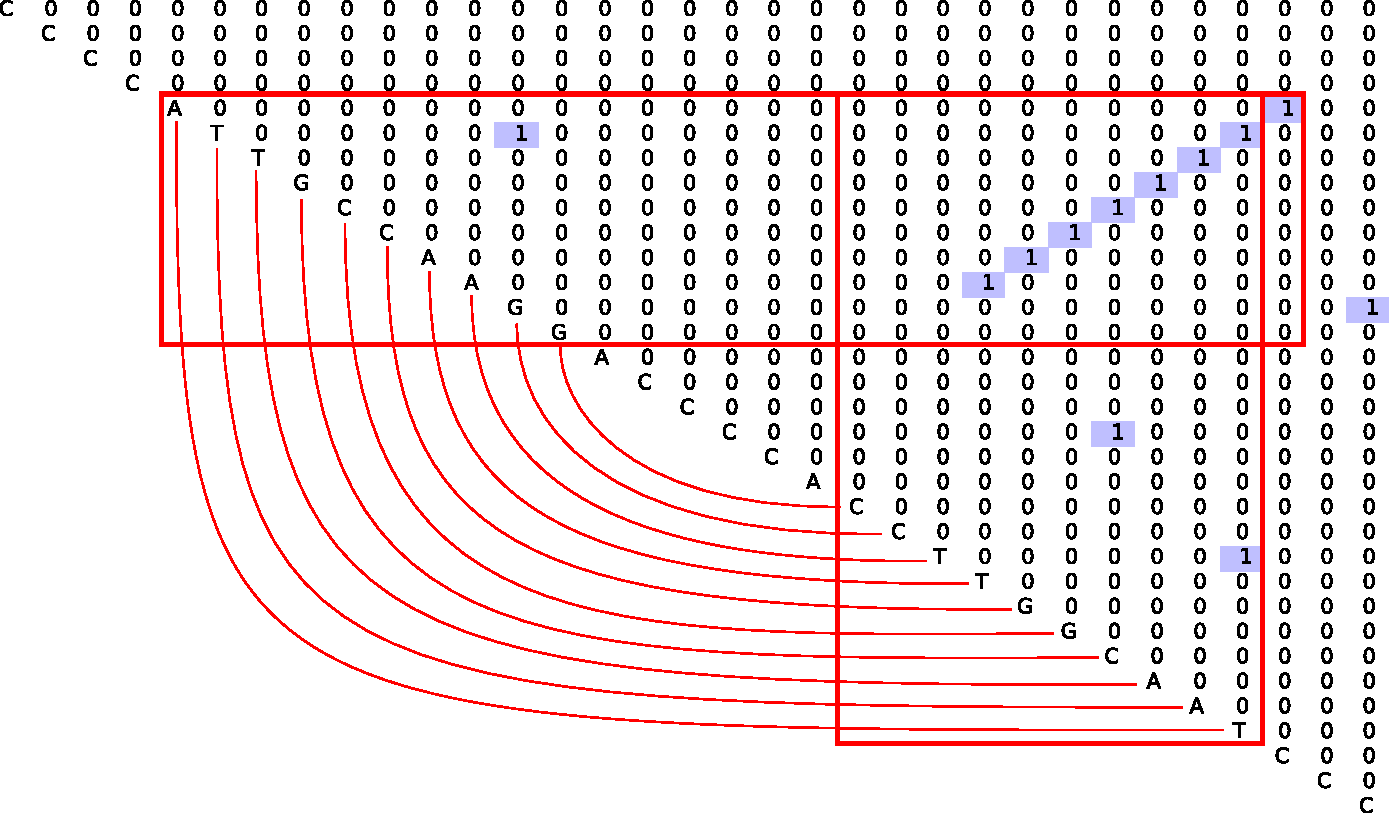
\includegraphics[width=0.8\textwidth]{figures/4.pdf}
\caption{Parsing result for sequence which should folds to
stem}
\label{fig:example}
\end{center}
\end{figure}

The result matrix can be linearized, compressed into byte or int vector, and handled by usind dense neural network, as described in~\cite{grigorevcomposition}.
But linearization brokes data locality: chain of ones which meens a high stem is local in terms of matrix, but be broken during its linearization.
It is the reason to investigate applicability of convolutional networks for parsing result handling: boolean natrix can be converted to black-white bitmap image.
In this work we provide empirical comparison of networks wich handle vectors and images.

Another problem is a bad performance of solution which is based on proposed approach.
As far as trained network handles parsing result, we should parse each sequence which we want ot process.
And parsig is a very time-consumption step: context-free parsing has cubic cimplexity in terms of input length.
Even if we use matrix-based parsing algorithm~\cite{Azimov:2018:CPQ:3210259.3210264} which utilizes GPGPU, performance is bad.
So, in practice it wolud be better to avoid parsing step.
In this work we propose a solution of this problem.
We show, how to build network which handles sequences, not parsing result.

\section{\bf The solution}

The first idea is to explore different formats of the parsing results representation and develop corresponding neural network architectures. The second idea is to minimize the use of parsing in the context of our solution.

We use such matrices as an input to neural network that is supposed to perform classification of some kind by detecting sufficient features and finding patterns in their appearance.
Therefore, we need to transform these boolean matrices to some data structures accepted by neural network.
Presently, we came up with two possible ways.
The first one is to drop out the bottom left triangle, vectorize it row by row and transform it to the byte vector.
This approach reduces the input size, but it requires the equal length of the input sequences, therefore we propose to either cut sequences or add some special symbol for each of them till the definite length.
The second way is to represent the matrix as an image: the false bits of matrix as white pixels and the true bits as black ones.
This approach makes it possible to process sequences with different length since the images could be easily transformed to a constant size.

The final step is to process the parsing-provided data by an artificial neural network constructed and trained for a specific task.
The neural network architecture is unique for each problem, but during the experimental research we worked out some common concepts.
For vectorized data we use dense layers because data locality is broken during vectorization and dropout layers with batch normalization to stabilize learning.
For image data we use a small number of convolutional layers, then linearization and go to the same architecture as for vectorized data, because convolution layers are suited for features extraction, but in our case it is already done by parsing.
In the previous work we performed experiments only on vectorized data and in this work we provide an evaluation on both data formats and compare the results.

To solve this problem we propose to use two-staged learning: to create a network we should first train another network wich solve subtask and after that use pretrained layers in final network.
In our case, firstly, we train a neural network which handles parsing results that performs classification according to a given problem.
After that, we extend this neural network by a number of input layers that take the initial nucleotide sequence as an inputs and convert it to the parsing result which handelas appropriately by pretarined layers.

So, we build a model that handles sequences and requires parsing only for training the model it is based on.
This way we can remove the parsing step from the usage of trained model and also improve its accuracy without the additional data generation.

In the next section we provide the results of this modification usage.


\section{\bf Experiments}

We evaluate the proposed approach with described above modifications on two tRNA sequences analysis tasks.
The first one is a classification of tRNA into two classes: eukaryotes and prokaryotes.
And the second one is a classification into four classes: archaea, bacteria, plants and fungi.
For these experiments we use sequences from tRNA databases~\cite{trnadb1,trnadb2}.
For both classification tasks we select the equal number of samples for each class and generated vectors and images datasets by parsing tool on the same sequences dataset using grammar presented in our previous work.
After that, we train neural networks that handle different representations of parsing results: vectors or images.
Then, for both vector- and image-based models we create the extended neural network which contains two blocks: the first one takes initial tRNA sequence as an input and transforms it to the parsing result by a number of dense layers with batch normalization and the second one is a block of pretrained layers from the base model which is created at the previos step.

These neural networks for two classes classification are shown in the figure~\ref{nn}, where the right rectangle represents model that handles vectors, the left rectangle represents network which classifies images and the middle rectangle here is the extension that transforms sequence to parsing result. For vector-based approach we combine this extension and the whole original sequence of layers.
For image-based approach we use the similar architecture, except in that case we remove the convolutional layer from the extended model, thus, at the junction of the blocks the first layer corresponds to linearized image.

\begin{figure}[h]
\begin{center}
\centering
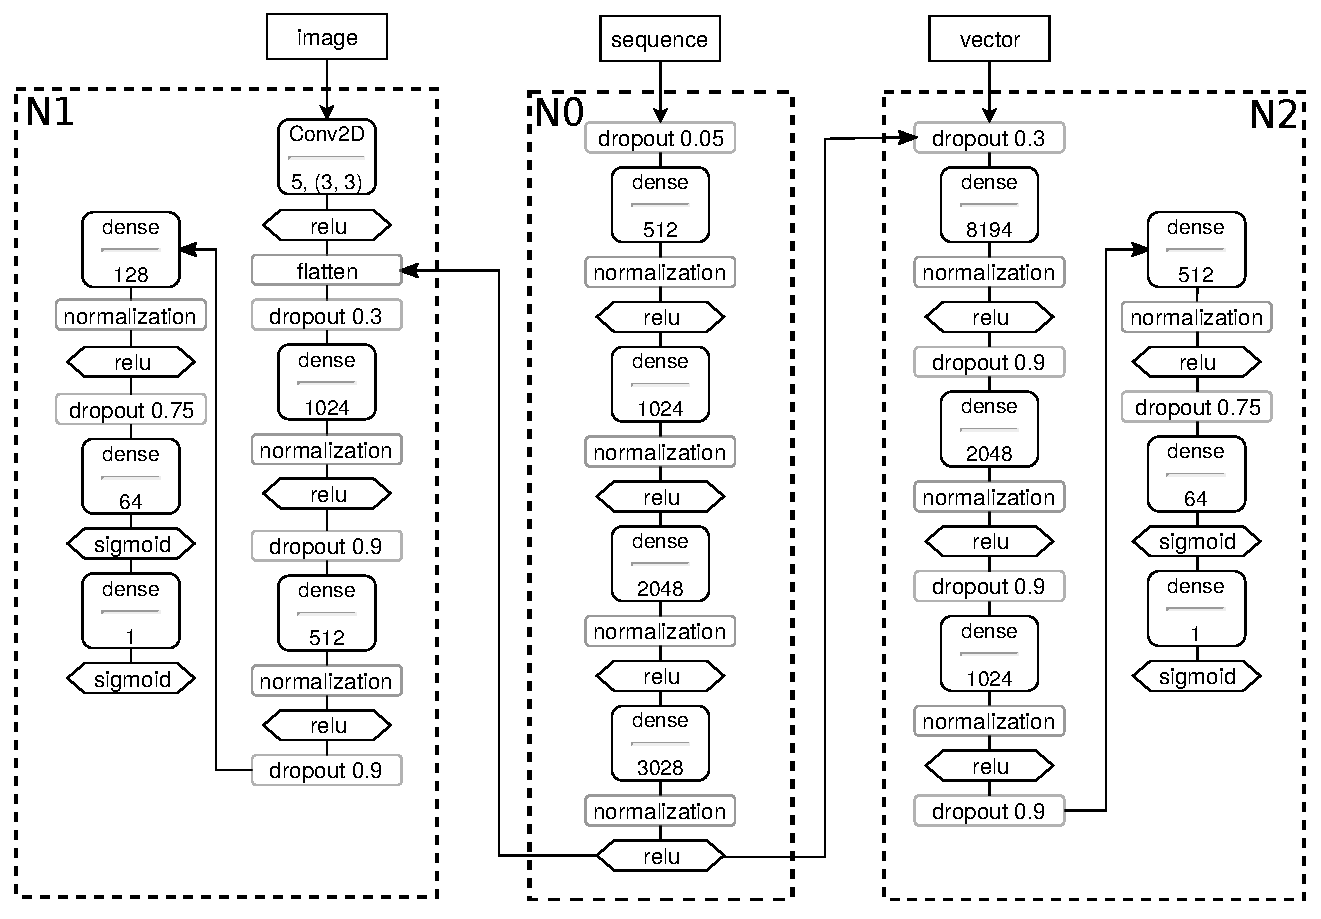
\includegraphics[width=14cm]{nn_arch.pdf}
\caption{Neural networks architectures}
\label{nn}
\end{center}
\end{figure}


All extended neural networks were trained and tested on the same datasets as the corresponding base ones. The trained models for two classes (EP) and for four classes (ABFP) classification tasks were estimated by using classical machine learning metrics: accuracy, precision and recall.

Results on test dataset for each problem by accuracy metrics are presented in the table~\ref{acc}, where base model is a model which handles parsing result (image or vector respectively) and extended model handles tRNA sequences and extends the corresponding base model.

\begin{table}[h]
\centering
\caption{Base and extended models test results by accuracy metrics}
\begin{tabular}{|l||l|l||l|l|}
\hline
Classifier                                                               & \multicolumn{2}{l||}{EP}               & \multicolumn{2}{l|}{ABFP}           \\ \hline \hline
Approach                                                                 & Vector-based       & Image-based      & Vector-based      & Image-based     \\ \hline
\begin{tabular}[c]{@{}l@{}}Base model\\ accuracy\end{tabular}            & 94.1\%             & 96.2\%           & 86.7\%            & 93.3\%          \\ \hline
\begin{tabular}[c]{@{}l@{}}Extended model \\ accuracy\end{tabular}       & 97.5\%             & 97.8\%           & 96.2\%            & 95.7\%          \\ \hline
\begin{tabular}[c]{@{}l@{}}Total training \\ time\end{tabular}       & 30000s             & 4600s           & 31800s            & 3600s          \\ \hline
\begin{tabular}[c]{@{}l@{}}Samples for\\ train:valid:test\end{tabular} & \multicolumn{2}{l||}{\begin{tabular}[c]{@{}l@{}}20000:5000:10000\\ (57\%:14\%:29\%)\end{tabular}} & \multicolumn{2}{l|}{\begin{tabular}[c]{@{}l@{}}8000:1000:3000\\ (67\%:8\%:25\%)\end{tabular}} \\ \hline
\end{tabular}
\label{acc}
\end{table}


Test results for extended models for both classifiers on the same amount of samples as in table~\ref{acc} by precision and recall metrics are presented in the table~\ref{pe}.

\begin{table}[h]
\centering
\caption{Models test results by precision and recall metrics for each class}
\begin{tabular}{|l||l|l|l|l|l|}
\hline
\multirow{2}{*}{Classifier} & \multirow{2}{*}{Class} & \multicolumn{2}{l|}{Vector-based approach} & \multicolumn{2}{l|}{Image-based approach} \\ \cline{3-6} 
                            &                        & precision         & recall        & precision        & recall        \\ \hline \hline
\multirow{2}{*}{EP}         & prokaryotic            & 95.8\%            & 99.4\%        & 96.2\%           & 99.4\%        \\ \cline{2-6} 
                            & eukaryotic             & 99.4\%            & 95.6\%        & 99.4\%           & 99.5\%        \\ \hline \hline
\multirow{4}{*}{ABFP}       & archaeal               & 91.1\%            & 99.2\%        & 91.6\%           & 98.5\%        \\ \cline{2-6} 
                            & bacterial              & 96.6\%            & 95.1\%        & 95.2\%           & 95.5\%        \\ \cline{2-6} 
                            & fungi                  & 98.5\%            & 94.9\%        & 97.5\%           & 94.3\%        \\ \cline{2-6} 
                            & plant                  & 99.4\%            & 95.7\%        & 99.2\%           & 94.7\%        \\ \hline
\end{tabular}
\label{pe}
\end{table}

The results show that our approach is applicable to tRNA classification tasks and both vector- and image-based models can be used along with dense and convolutional layers in neural networks architectures.
While the differences in results for extended models are insignificant, for base models image-based network demonstrates slightly better results (see table~\ref{acc}).
The reason of this effect may be a better locality of features in the image-based representation of parsing result: chain of ones which means a high stem is local in terms of picture, but can be broken during linearization.
In the current model, we use only one convolution layer.
Whether it is possible to utilize deep convolutional networks for secondary structure analysis in the discussed approach is a question for future research.

The idea of extended model that handles sequences instead of parsing result is proved to be applicable in practice and it demonstrates even higher quality than the original parsing-based model, as it can be seen in the table~\ref{acc}.
We can conclude that it is possible to use parsing only for network training without loss of network quality.

\section{\bf Conclusion}

We describe modifications of the proposed approach for biological sequences analysis using the combination of formal grammars and neural networks.
We show that it is possible to handle parsing result which is represented as an image by using convolutional layers while processing it with a neural network, and this way it is possible to improve quality of the solution.
Also, we provide a solution that removes the parsing step from the trained model use and allows to run models on the original RNA sequences.
As a result, the performance of the final solution can be significantly improved.
We demonstrated the applicability of the proposed modifications for real-world problems.
Source code and documentation are published at GitHub: \url{https://github.com/LuninaPolina/SecondaryStructureAnalyzer}.

We can provide a number of directions for future research.
First of all, it is necessary to investigate the applicability of the proposed approach for other sequences processing and for other tasks.
For examples, for 16s rRNA processing, and for chimeric sequences filtration.

Another possible application is a secondary structure prediction.
Is it possible to create a generative network which generates the most possible contact map for the given sequence?

The image-based model demonstrates a slightly higher quality.
We should investigate this effect.
We think that the reason is a better locality of features.
If so, it should be possible the create deep convolution network for secondary structure analysis.

Finally, it is important to find a theoretical base for grammar tuning. Is it possible to use theoretical results on secondary structure description by using formal grammar, such as~\cite{MQbioinformatics19} to find optimal grammar for our approach?


\section*{\bf Acknowledgments}

The research was supported by the Russian Science Foundation grant 18-11-00100 and a grant from JetBrains Research.



%\bibliographystyle{apalike}
\bibliographystyle{ieeetr}

{\fontsize{10}{10}\selectfont
%\begin{thebibliography}{99}
\setlength{\parskip}{0pt}

\bibliography{main}

%\end{thebibliography}
}
\end{document}
